\documentclass{article}
\usepackage{geometry}
\geometry{margin=1in}
\usepackage{tikz}
\usepackage{amssymb}

% fleqn allows setting indent of display math
\usepackage[fleqn]{amsmath}
\setlength{\mathindent}{0pt} % Set indent
% Disable equation numbering (https://tex.stackexchange.com/a/360378)
\makeatletter
\renewcommand\tagform@[1]{}
\makeatother
% Disable page numbering (https://tex.stackexchange.com/a/360378)
\makeatletter
\renewcommand\tagform@[1]{}
\makeatother

% Allow Unicode (some, e.g., © and £ at least)
% https://tex.stackexchange.com/questions/370278/is-there-any-reason-to-use-inputenc
\usepackage[utf8]{inputenc}

% Hyperlinks
\usepackage{hyperref}
\hypersetup{colorlinks=true, urlcolor=blue, linkcolor=blue}

% Prevent indentation of paragraphs
\setlength\parindent{0pt}
\setlength{\parskip}{\baselineskip}

% Spacing above/below equations
% https://tex.stackexchange.com/a/69678
\AtBeginDocument{%
 \abovedisplayskip=-\parskip
 \abovedisplayshortskip=-\parskip
 \belowdisplayskip=0em
 \belowdisplayshortskip=0em
}

% Allow 3 additional subsection levels
% https://tex.stackexchange.com/a/60212
\usepackage{titlesec}
\setcounter{secnumdepth}{6}
% H4 in HTML
\titleformat{\paragraph}{\normalfont\normalsize\bfseries}{\theparagraph}{1em}{}
\titlespacing*{\paragraph}{0pt}{3.25ex plus 1ex minus .2ex}{1.5ex plus .2ex}
% H5 in HTML
\titleformat{\subparagraph}{\normalfont\normalsize\bfseries}{\thesubparagraph}{1em}{}
\titlespacing*{\subparagraph}{0pt}{3.25ex plus 1ex minus .2ex}{1.5ex plus .2ex}
% H6 in HTML
\titleformat{\subsubparagraph}{\normalfont\normalsize\bfseries}{\thesubsubparagraph}{1em}{}
\titlespacing*{\subsubparagraph}{0pt}{3.25ex plus 1ex minus .2ex}{1.5ex plus .2ex}


\renewcommand{\mbox}{\text}
\newcommand{\ds}[0]{\displaystyle}
\newcommand{\ihat}[0]{\hat{\boldsymbol{\imath}}}
\newcommand{\jhat}[0]{\hat{\boldsymbol{\jmath}}}
\newcommand{\khat}[0]{\hat{\boldsymbol{k}}}
\newcommand{\xhat}[0]{\hat{\mathbf{x}}}
\newcommand{\yhat}[0]{\hat{\mathbf{y}}}
\newcommand{\zhat}[0]{\hat{\mathbf{z}}}
\newcommand{\rhat}[0]{\hat{\mathbf{r}}}
\newcommand{\bfvec}[1]{\vec{\mathbf{#1}}}
\newcommand{\bfcdot}[0]{\boldsymbol{\cdot}}

\usepackage{fancyhdr}
\pagestyle{fancy}
\lhead{Electric Flux}
\rhead{\thepage}

\begin{document}

\section{Overview}

Several calculations must be performed to use Gauss's law to find the electric field for a system of charges (if possible). First, one must find the electric flux through a closed surface. Second, one must find the amount of charge inside of a closed surface. In this activity, you will compute the electric flux through both open and closed surfaces.

Electric flux, $\Phi_E$, is the integral of $\bfvec{E}\bfcdot d\bfvec{A}$ over a surface: 

\begin{equation}
\Phi_E=\int\bfvec{E}\bfcdot d\bfvec{A}
\end{equation}

When the magnitude and direction of $\bfvec{E}$ is the same at all points on the surface, the integral simplifies to 

\begin{equation}
\Phi_E = \bfvec{E}\bfcdot \bfvec{A} = \bfvec{E}\bfcdot \hat{\mathbf{n}}A
\end{equation}

where $\hat{\mathbf{n}}$ is a unit vector that is perpendicular to the surface with area $A$. Electric flux is a scalar quantity because it results from the dot product of two vectors (similar to work, which is the dot product of a force vector and displacement vector).

The equation $\Phi_E = \bfvec{E}\bfcdot \hat{\mathbf{n}}A$ can also be written as

\begin{equation}
\Phi_E = E_{\perp}A
\end{equation}

where $E_{\perp}$ is the component of $\bfvec{E}$ that is perpendicular to $A$. If the perpendicular component of $\bfvec{E}$ is in the same direction as the normal direction for $\bfvec{A}$, the flux is positive. If the perpendicular component of $\bfvec{E}$ is in the opposite direction as the normal direction for $\bfvec{A}$, the flux is negative.

\newpage

\section{$\Phi_E$ Through Open Surface}

\subsection{Problem I}



\tikzset{every picture/.style={line width=0.75pt}} %set default line width to 0.75pt        

\begin{tikzpicture}[x=0.75pt,y=0.75pt,yscale=-1,xscale=1]
%uncomment if require: \path (0,194); %set diagram left start at 0, and has height of 194

%Straight Lines [id:da811311968505924] 
\draw [color={rgb, 255:red, 0; green, 0; blue, 255 }  ,draw opacity=1 ] [dash pattern={on 0.84pt off 2.51pt}]  (30,158.27) -- (30,78.27) ;
%Straight Lines [id:da7313799653634994] 
\draw    (70,118.27) -- (11.41,176.85) ;
\draw [shift={(10,178.27)}, rotate = 315] [color={rgb, 255:red, 0; green, 0; blue, 0 }  ][line width=0.75]    (10.93,-3.29) .. controls (6.95,-1.4) and (3.31,-0.3) .. (0,0) .. controls (3.31,0.3) and (6.95,1.4) .. (10.93,3.29)   ;
%Straight Lines [id:da29883780704593876] 
\draw    (70,118.27) -- (168,118.27) ;
\draw [shift={(170,118.27)}, rotate = 180] [color={rgb, 255:red, 0; green, 0; blue, 0 }  ][line width=0.75]    (10.93,-3.29) .. controls (6.95,-1.4) and (3.31,-0.3) .. (0,0) .. controls (3.31,0.3) and (6.95,1.4) .. (10.93,3.29)   ;
%Straight Lines [id:da11080156820767506] 
\draw    (70,38.27) -- (70,16.47) ;
\draw [shift={(70,14.47)}, rotate = 90] [color={rgb, 255:red, 0; green, 0; blue, 0 }  ][line width=0.75]    (10.93,-3.29) .. controls (6.95,-1.4) and (3.31,-0.3) .. (0,0) .. controls (3.31,0.3) and (6.95,1.4) .. (10.93,3.29)   ;
%Straight Lines [id:da5176231657951886] 
\draw [color={rgb, 255:red, 0; green, 0; blue, 255 }  ,draw opacity=1 ] [dash pattern={on 0.84pt off 2.51pt}]  (70,38.27) -- (30,78.27) ;
%Straight Lines [id:da3712391591803177] 
\draw [color={rgb, 255:red, 0; green, 0; blue, 255 }  ,draw opacity=1 ]   (70,118.27) -- (70,38.27) ;
%Straight Lines [id:da11750921868597053] 
\draw [color={rgb, 255:red, 0; green, 0; blue, 255 }  ,draw opacity=1 ] [dash pattern={on 0.84pt off 2.51pt}]  (70,118.27) -- (30,158.27) ;
%Straight Lines [id:da088451068717462] 
\draw [color={rgb, 255:red, 255; green, 0; blue, 0 }  ,draw opacity=1 ] [dash pattern={on 0.84pt off 2.51pt}]  (71,38.27) -- (71,118.27) ;
%Straight Lines [id:da08941496830503048] 
\draw    (29,158.27) -- (35,158.27) ;
%Straight Lines [id:da1991772887887806] 
\draw    (64,38.27) -- (71,38.27) ;

% Text Node
\draw (15,175.67) node [anchor=north west][inner sep=0.75pt]    {$x$};
% Text Node
\draw (156,126.67) node [anchor=north west][inner sep=0.75pt]    {$y$};
% Text Node
\draw (75.25,12.4) node [anchor=north west][inner sep=0.75pt]    {$z$};
% Text Node
\draw (35,153.67) node [anchor=north west][inner sep=0.75pt]  [font=\scriptsize]  {$x_{o}$};
% Text Node
\draw (47,30.67) node [anchor=north west][inner sep=0.75pt]  [font=\scriptsize]  {$z_{o}$};


\end{tikzpicture}


\begin{enumerate}

  \item a. Draw an area vector $\bfvec{A}=\hat{\mathbf{n}}A$ on the figure.\\

        b. Is there only one normal direction to this area? Discuss your reasoning with your group.

\end{enumerate}

\begin{enumerate}

  \item[2.] For each of the following $\bfvec{E}$, draw  $\bfvec{E}$ and $\hat{\mathbf{n}}$ for the area in the previous figure when viewed from a point on the positive $z$-axis that is far from the origin (that is, draw the projection onto the $x$--$y$ plane). Then compute $\Phi_E$.\\

            a. $\bfvec{E}=E_o\ihat\qquad$ $\Phi_E=$\\

            b. $\bfvec{E}=E_o\jhat\qquad$ $\Phi_E=$\\

            c. $\bfvec{E}=E_o\khat\qquad$ $\Phi_E=$\\

            d. $\bfvec{E}=E_o\ihat + E_o\jhat\qquad$ $\Phi_E=$

\end{enumerate}

\begin{enumerate}

  \item[3.] For each of the cases in 2., what is $E_{\perp}$ (the component of $\bfvec{E}$ that is perpendicular to the surface)? Also compute $\Phi_E=E_{\perp}A$.\\

            a. $E_{\perp}=\qquad$ $\Phi_E=E_{\perp}A=$\\

            b. $E_{\perp}=\qquad$ $\Phi_E=E_{\perp}A=$\\

            c. $E_{\perp}=\qquad$ $\Phi_E=E_{\perp}A=$\\

            d. $E_{\perp}=\qquad$ $\Phi_E=E_{\perp}A=$

\end{enumerate}

\newpage

\subsection{Problem II}



\tikzset{every picture/.style={line width=0.75pt}} %set default line width to 0.75pt        

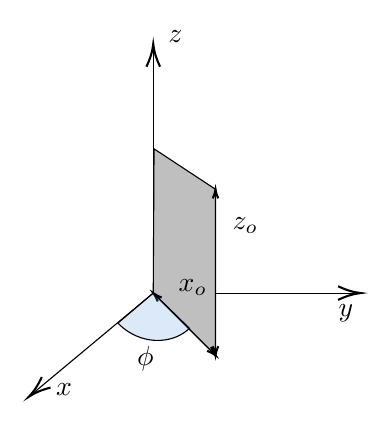
\begin{tikzpicture}[x=0.75pt,y=0.75pt,yscale=-1,xscale=1]
%uncomment if require: \path (0,193); %set diagram left start at 0, and has height of 193

%Straight Lines [id:da3344454963441721] 
\draw    (70,12) -- (70,130) ;
\draw [shift={(70,10)}, rotate = 90] [color={rgb, 255:red, 0; green, 0; blue, 0 }  ][line width=0.75]    (10.93,-3.29) .. controls (6.95,-1.4) and (3.31,-0.3) .. (0,0) .. controls (3.31,0.3) and (6.95,1.4) .. (10.93,3.29)   ;
%Shape: Polygon [id:ds46480537066610883] 
\draw  [fill={rgb, 255:red, 155; green, 155; blue, 155 }  ,fill opacity=0.64 ] (70,130) -- (100,160) -- (100,80) -- (70.38,60.5) -- cycle ;
%Straight Lines [id:da17740345654787837] 
\draw    (71.41,131.41) -- (98.59,158.59) ;
\draw [shift={(100,160)}, rotate = 225] [color={rgb, 255:red, 0; green, 0; blue, 0 }  ][line width=0.75]    (4.37,-1.32) .. controls (2.78,-0.56) and (1.32,-0.12) .. (0,0) .. controls (1.32,0.12) and (2.78,0.56) .. (4.37,1.32)   ;
\draw [shift={(70,130)}, rotate = 45] [color={rgb, 255:red, 0; green, 0; blue, 0 }  ][line width=0.75]    (4.37,-1.32) .. controls (2.78,-0.56) and (1.32,-0.12) .. (0,0) .. controls (1.32,0.12) and (2.78,0.56) .. (4.37,1.32)   ;
%Straight Lines [id:da1611967621487418] 
\draw    (100,82) -- (100,158) ;
\draw [shift={(100,160)}, rotate = 270] [color={rgb, 255:red, 0; green, 0; blue, 0 }  ][line width=0.75]    (4.37,-1.32) .. controls (2.78,-0.56) and (1.32,-0.12) .. (0,0) .. controls (1.32,0.12) and (2.78,0.56) .. (4.37,1.32)   ;
\draw [shift={(100,80)}, rotate = 90] [color={rgb, 255:red, 0; green, 0; blue, 0 }  ][line width=0.75]    (4.37,-1.32) .. controls (2.78,-0.56) and (1.32,-0.12) .. (0,0) .. controls (1.32,0.12) and (2.78,0.56) .. (4.37,1.32)   ;
%Straight Lines [id:da5493760744821823] 
\draw    (70,130) -- (11.54,178.72) ;
\draw [shift={(10,180)}, rotate = 320.19] [color={rgb, 255:red, 0; green, 0; blue, 0 }  ][line width=0.75]    (10.93,-3.29) .. controls (6.95,-1.4) and (3.31,-0.3) .. (0,0) .. controls (3.31,0.3) and (6.95,1.4) .. (10.93,3.29)   ;
%Straight Lines [id:da2795261006841576] 
\draw    (100,130) -- (168,130) ;
\draw [shift={(170,130)}, rotate = 180] [color={rgb, 255:red, 0; green, 0; blue, 0 }  ][line width=0.75]    (10.93,-3.29) .. controls (6.95,-1.4) and (3.31,-0.3) .. (0,0) .. controls (3.31,0.3) and (6.95,1.4) .. (10.93,3.29)   ;
%Shape: Pie [id:dp974067234639628] 
\draw  [fill={rgb, 255:red, 74; green, 144; blue, 226 }  ,fill opacity=0.2 ] (87.48,147.01) .. controls (80.15,153.89) and (68.11,154.89) .. (58.3,148.79) .. controls (56.29,147.54) and (54.51,146.07) .. (52.97,144.45) -- (70,130) -- cycle ;

% Text Node
\draw (81,122.4) node [anchor=north west][inner sep=0.75pt]    {$x_{o}$};
% Text Node
\draw (22,172.4) node [anchor=north west][inner sep=0.75pt]    {$x$};
% Text Node
\draw (158,134.4) node [anchor=north west][inner sep=0.75pt]    {$y$};
% Text Node
\draw (76,2.4) node [anchor=north west][inner sep=0.75pt]    {$z$};
% Text Node
\draw (107,92.4) node [anchor=north west][inner sep=0.75pt]    {$z_{o}$};
% Text Node
\draw (61,154.4) node [anchor=north west][inner sep=0.75pt]    {$\phi $};


\end{tikzpicture}


If the area from the previous problem is rotated by $\phi=45^\circ$ around the $z$--axis, compute the flux for each electric field. Hint: Draw the area as it would look from a point on the positive $z$-axis that is far from the origin (that is, draw the projection onto the $x$--$y$ plane). Then draw $\hat{\mathbf{n}}$ and $\bfvec{E}$ for each case.

   a. $\bfvec{E}=E_o\ihat\qquad$ $\Phi_E=$

   b. $\bfvec{E}=E_o\jhat\qquad$ $\Phi_E=$ 

   c. $\bfvec{E}=E_o\khat\qquad$ $\Phi_E=$ 

   d. $\bfvec{E}=E_o\ihat + E_o\jhat\qquad$ $\Phi_E=$

\section{$\Phi_E$ Through Closed Surface}

In the previous problem, you computed the flux through an open surface. You should have noted that one can associate two area vectors to an open surface -- imagine your hand being an open surface. You can put the a pencil (1) on the top of your hand with the tip pointing up or (2) in your palm with the tip pointing down. The pencil represents the vector and the tip indicates the direction.

Gauss's law, which involves electric flux, always involves a closed surface (if you put water inside a closed surface, it would not leak out). For Gauss's law, there is a convention for which area vector to choose -- it is the one that points outwards from the volume that the surface encloses. 

In the following example, the electric flux is computed through a closed surface (a cube) by finding the flux through each of the faces of the cube. The total electric flux is the sum of the fluxes though each cube.

%The reason that we are interested in knowing the flux through a closed surface is due to a remarkable mathematical result known as Gauss's law. Suppose that you are able to measure the electric field on an arbitrary and closed surface. The net electric flux through the surface that you compute is related to the total amount of charge inside the surface! For example, if you are given the electric field at all points on the surface of a closed cardboard box, you can compute the total charge inside the box without having to open it. 

With Coulomb's law, we are given the location and values of charges and we compute the electric field anywhere in space. With Gauss's law, we can do the reverse -- given an electric field on the surface of a small volume of space, we can compute the charge in the volume. (If the volume is large, we can only compute the amount of charge enclosed in the volume; however, if the closed surface volume approaches zero, we can compute the amount of charge at a point in space.)

\newpage

\subsection{Example}



\tikzset{every picture/.style={line width=0.75pt}} %set default line width to 0.75pt        

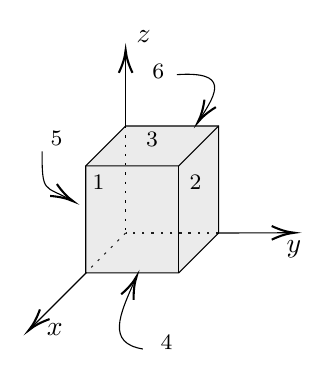
\begin{tikzpicture}[x=0.75pt,y=0.75pt,yscale=-1,xscale=1]
%uncomment if require: \path (0,177); %set diagram left start at 0, and has height of 177

%Straight Lines [id:da6367799622029096] 
\draw  [dash pattern={on 0.84pt off 2.51pt}]  (71.2,110.8) -- (52,130) ;
%Straight Lines [id:da6001535337839026] 
\draw  [dash pattern={on 0.84pt off 2.51pt}]  (116,110.8) -- (71.2,110.8) ;
%Shape: Cube [id:dp04342558315379508] 
\draw  [fill={rgb, 255:red, 155; green, 155; blue, 155 }  ,fill opacity=0.2 ] (52,78.45) -- (71.2,59.25) -- (116,59.25) -- (116,110.8) -- (96.8,130) -- (52,130) -- cycle ; \draw   (116,59.25) -- (96.8,78.45) -- (52,78.45) ; \draw   (96.8,78.45) -- (96.8,130) ;
%Straight Lines [id:da33768233880307563] 
\draw  [dash pattern={on 0.84pt off 2.51pt}]  (71.2,59.25) -- (71.2,110.8) ;
%Straight Lines [id:da8556566864205468] 
\draw    (52.17,130) -- (25.91,156.25) ;
\draw [shift={(24.5,157.67)}, rotate = 315] [color={rgb, 255:red, 0; green, 0; blue, 0 }  ][line width=0.75]    (10.93,-3.29) .. controls (6.95,-1.4) and (3.31,-0.3) .. (0,0) .. controls (3.31,0.3) and (6.95,1.4) .. (10.93,3.29)   ;
%Straight Lines [id:da7859931310096506] 
\draw    (116,110.8) -- (150.5,110.67) ;
\draw [shift={(152.5,110.67)}, rotate = 179.79] [color={rgb, 255:red, 0; green, 0; blue, 0 }  ][line width=0.75]    (10.93,-3.29) .. controls (6.95,-1.4) and (3.31,-0.3) .. (0,0) .. controls (3.31,0.3) and (6.95,1.4) .. (10.93,3.29)   ;
%Straight Lines [id:da7670470282458908] 
\draw    (71.2,59.25) -- (71.2,24.67) ;
\draw [shift={(71.2,22.67)}, rotate = 90] [color={rgb, 255:red, 0; green, 0; blue, 0 }  ][line width=0.75]    (10.93,-3.29) .. controls (6.95,-1.4) and (3.31,-0.3) .. (0,0) .. controls (3.31,0.3) and (6.95,1.4) .. (10.93,3.29)   ;
%Curve Lines [id:da43558820809067944] 
\draw    (79.5,166.67) .. controls (62.04,163.76) and (68.1,150.5) .. (75.78,133.28) ;
\draw [shift={(76.5,131.67)}, rotate = 113.96] [color={rgb, 255:red, 0; green, 0; blue, 0 }  ][line width=0.75]    (10.93,-3.29) .. controls (6.95,-1.4) and (3.31,-0.3) .. (0,0) .. controls (3.31,0.3) and (6.95,1.4) .. (10.93,3.29)   ;
%Curve Lines [id:da8847199212806154] 
\draw    (30.93,71.49) .. controls (30.93,91.65) and (31.85,87.85) .. (44.31,94.59) ;
\draw [shift={(45.93,95.49)}, rotate = 209.74] [color={rgb, 255:red, 0; green, 0; blue, 0 }  ][line width=0.75]    (10.93,-3.29) .. controls (6.95,-1.4) and (3.31,-0.3) .. (0,0) .. controls (3.31,0.3) and (6.95,1.4) .. (10.93,3.29)   ;
%Curve Lines [id:da0524228217917051] 
\draw    (95.93,34.49) .. controls (120.89,32.85) and (115.44,42.92) .. (107,55.86) ;
\draw [shift={(105.93,57.49)}, rotate = 303.27] [color={rgb, 255:red, 0; green, 0; blue, 0 }  ][line width=0.75]    (10.93,-3.29) .. controls (6.95,-1.4) and (3.31,-0.3) .. (0,0) .. controls (3.31,0.3) and (6.95,1.4) .. (10.93,3.29)   ;

% Text Node
\draw (54,81.85) node [anchor=north west][inner sep=0.75pt]  [font=\footnotesize]  {$1$};
% Text Node
\draw (100.8,81.85) node [anchor=north west][inner sep=0.75pt]  [font=\footnotesize]  {$2$};
% Text Node
\draw (79.87,60.77) node [anchor=north west][inner sep=0.75pt]  [font=\footnotesize,rotate=-0.7]  {$3$};
% Text Node
\draw (32,153.4) node [anchor=north west][inner sep=0.75pt]    {$x$};
% Text Node
\draw (147.5,113.07) node [anchor=north west][inner sep=0.75pt]    {$y$};
% Text Node
\draw (86.87,158.77) node [anchor=north west][inner sep=0.75pt]  [font=\footnotesize,rotate=-0.7]  {$4$};
% Text Node
\draw (33.87,60.42) node [anchor=north west][inner sep=0.75pt]  [font=\footnotesize,rotate=-0.7]  {$5$};
% Text Node
\draw (75.25,12.13) node [anchor=north west][inner sep=0.75pt]    {$z$};
% Text Node
\draw (82.87,28.42) node [anchor=north west][inner sep=0.75pt]  [font=\footnotesize,rotate=-0.7]  {$6$};


\end{tikzpicture}


Find the flux through the six labeled faces of the cube with side length $a$ when the electric field is everywhere in the $+z$ direction with magnitude $E_o$.

\textbf{Answer}

This example is similar to Example 22.2a of the textbook. We'll solve it using two methods. The first method is useful for cases when the electric field is either parallel or perpendicular to all surfaces. The second method is useful for more general cases, such as problem 3.3.

\textbf{Method I}

The electric field is parallel to surfaces 1, 2, 5, and 6. Thinking in terms of the analogy of the electric field representing lines of flow, the flux is zero through these faces. 

$\Phi_E^{1}=\Phi_E^{2}=\Phi_E^{5}=\Phi_E^{6}=0$

By convention, the normal direction for surface 3 is outwards from the volume, which is in the $+z$-direction. The electric field is in the same direction, so

$\Phi_E^{3}=E_oA=E_oa^2$

The normal direction for the bottom surface is downwards, which is in the opposite direction as the electric field, so

$\Phi_E^{4}=-E_oA=-E_oa^2$

The total flux through the cube, $\Phi_E^1+…+\Phi_E^6$, is zero. Thinking again in terms of the electric field representing flow lines, every electric field line that enters the cube exits, so the flow in equals the flow out. (Perhaps confusingly, flow out of a volume corresponds to a positive flux. The reason for this convention for flux is that from Gauss's law, a net positive flow out of a closed surface corresponds to a net positive charge inside the surface.)

\textbf{Method II}

In this problem, the normal vectors are parallel to the Cartesian unit vectors. Based on the diagram, $\hat{\mathbf{n}}_1=\ihat$, $\hat{\mathbf{n}}_2=\jhat$, $\hat{\mathbf{n}}_3=\khat$, $\hat{\mathbf{n}}_4=-\khat$
$\hat{\mathbf{n}}_5=-\jhat$, $\hat{\mathbf{n}}_6=-\ihat$. The negative sign for the last three normal vectors is due to the convention that the normal points outwards from a closed surface.

The area vector is the area times the normal vector, so $\bfvec{A}_1=A\ihat$, $\bfvec{A}_2=A\jhat$, $\bfvec{A}_3=A\khat$, $\bfvec{A}_4=-A\khat$, $\bfvec{A}_4=-A\jhat$, and $\bfvec{A}_4=-A\ihat$, where $A=a^2$.

Recall that $\ihat\cdot\ihat=\jhat\cdot\jhat=\khat\cdot\khat=1$ and the dot product of any other combinations of Cartesian unit vectors is zero: $\ihat\cdot\jhat=0$, $\jhat\cdot\khat=0$, and $\ihat\cdot\khat=0$. Dot products of unit vectors are reviewed in Section 1.10 of the textbook.

$\Phi_E^{1}=\bfvec{E}\cdot \bfvec{A}_1=\bfvec{E}\cdot A\hat{\mathbf{n}}_1=E_o\khat\cdot A\ihat=E_oA(\khat\cdot \ihat)=0$

$\Phi_E^{2}=\bfvec{E}\cdot \bfvec{A}_2=\bfvec{E}\cdot A\hat{\mathbf{n}}_2=E_o\hat{\mathbf{k}}\cdot A\jhat=E_oA(\khat\cdot \jhat)=0$

$\Phi_E^{3}=\bfvec{E}\cdot \bfvec{A}_3=\bfvec{E}\cdot A\hat{\mathbf{n}}_3=E_o\hat{\mathbf{k}}\cdot A\khat=E_oA(\khat\cdot\khat)=E_oA=E_oa^2$

$\Phi_E^{4}=\bfvec{E}\cdot \bfvec{A}_4=\bfvec{E}\cdot A\hat{\mathbf{n}}_4=E_o\hat{\mathbf{k}}\cdot (-A\khat)=-E_oA(\khat\cdot\khat)=-E_oa^2$

$\Phi_E^{5}=\bfvec{E}\cdot \bfvec{A}_5=\bfvec{E}\cdot A\hat{\mathbf{n}}_5=E_o\hat{\mathbf{k}}\cdot (-A\jhat)=E_oA(\khat\cdot\jhat)=0$

$\Phi_E^{6}=\bfvec{E}\cdot \bfvec{A}_6=\bfvec{E}\cdot A\hat{\mathbf{n}}_6=E_o\hat{\mathbf{k}}\cdot (-A\ihat)=-E_oA(\khat\cdot\ihat)=0$

How much charge is inside the cube? The net flux through the cube's surface is zero, so it follows from Gauss's law that the total charge enclosed is zero.

\newpage

\subsection{Problem}



\tikzset{every picture/.style={line width=0.75pt}} %set default line width to 0.75pt        

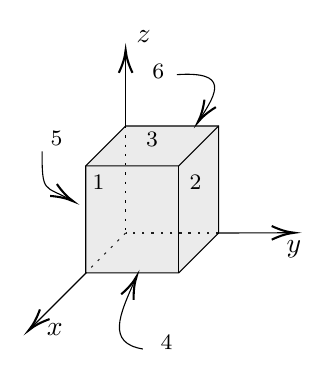
\begin{tikzpicture}[x=0.75pt,y=0.75pt,yscale=-1,xscale=1]
%uncomment if require: \path (0,177); %set diagram left start at 0, and has height of 177

%Straight Lines [id:da6367799622029096] 
\draw  [dash pattern={on 0.84pt off 2.51pt}]  (71.2,110.8) -- (52,130) ;
%Straight Lines [id:da6001535337839026] 
\draw  [dash pattern={on 0.84pt off 2.51pt}]  (116,110.8) -- (71.2,110.8) ;
%Shape: Cube [id:dp04342558315379508] 
\draw  [fill={rgb, 255:red, 155; green, 155; blue, 155 }  ,fill opacity=0.2 ] (52,78.45) -- (71.2,59.25) -- (116,59.25) -- (116,110.8) -- (96.8,130) -- (52,130) -- cycle ; \draw   (116,59.25) -- (96.8,78.45) -- (52,78.45) ; \draw   (96.8,78.45) -- (96.8,130) ;
%Straight Lines [id:da33768233880307563] 
\draw  [dash pattern={on 0.84pt off 2.51pt}]  (71.2,59.25) -- (71.2,110.8) ;
%Straight Lines [id:da8556566864205468] 
\draw    (52.17,130) -- (25.91,156.25) ;
\draw [shift={(24.5,157.67)}, rotate = 315] [color={rgb, 255:red, 0; green, 0; blue, 0 }  ][line width=0.75]    (10.93,-3.29) .. controls (6.95,-1.4) and (3.31,-0.3) .. (0,0) .. controls (3.31,0.3) and (6.95,1.4) .. (10.93,3.29)   ;
%Straight Lines [id:da7859931310096506] 
\draw    (116,110.8) -- (150.5,110.67) ;
\draw [shift={(152.5,110.67)}, rotate = 179.79] [color={rgb, 255:red, 0; green, 0; blue, 0 }  ][line width=0.75]    (10.93,-3.29) .. controls (6.95,-1.4) and (3.31,-0.3) .. (0,0) .. controls (3.31,0.3) and (6.95,1.4) .. (10.93,3.29)   ;
%Straight Lines [id:da7670470282458908] 
\draw    (71.2,59.25) -- (71.2,24.67) ;
\draw [shift={(71.2,22.67)}, rotate = 90] [color={rgb, 255:red, 0; green, 0; blue, 0 }  ][line width=0.75]    (10.93,-3.29) .. controls (6.95,-1.4) and (3.31,-0.3) .. (0,0) .. controls (3.31,0.3) and (6.95,1.4) .. (10.93,3.29)   ;
%Curve Lines [id:da43558820809067944] 
\draw    (79.5,166.67) .. controls (62.04,163.76) and (68.1,150.5) .. (75.78,133.28) ;
\draw [shift={(76.5,131.67)}, rotate = 113.96] [color={rgb, 255:red, 0; green, 0; blue, 0 }  ][line width=0.75]    (10.93,-3.29) .. controls (6.95,-1.4) and (3.31,-0.3) .. (0,0) .. controls (3.31,0.3) and (6.95,1.4) .. (10.93,3.29)   ;
%Curve Lines [id:da8847199212806154] 
\draw    (30.93,71.49) .. controls (30.93,91.65) and (31.85,87.85) .. (44.31,94.59) ;
\draw [shift={(45.93,95.49)}, rotate = 209.74] [color={rgb, 255:red, 0; green, 0; blue, 0 }  ][line width=0.75]    (10.93,-3.29) .. controls (6.95,-1.4) and (3.31,-0.3) .. (0,0) .. controls (3.31,0.3) and (6.95,1.4) .. (10.93,3.29)   ;
%Curve Lines [id:da0524228217917051] 
\draw    (95.93,34.49) .. controls (120.89,32.85) and (115.44,42.92) .. (107,55.86) ;
\draw [shift={(105.93,57.49)}, rotate = 303.27] [color={rgb, 255:red, 0; green, 0; blue, 0 }  ][line width=0.75]    (10.93,-3.29) .. controls (6.95,-1.4) and (3.31,-0.3) .. (0,0) .. controls (3.31,0.3) and (6.95,1.4) .. (10.93,3.29)   ;

% Text Node
\draw (54,81.85) node [anchor=north west][inner sep=0.75pt]  [font=\footnotesize]  {$1$};
% Text Node
\draw (100.8,81.85) node [anchor=north west][inner sep=0.75pt]  [font=\footnotesize]  {$2$};
% Text Node
\draw (79.87,60.77) node [anchor=north west][inner sep=0.75pt]  [font=\footnotesize,rotate=-0.7]  {$3$};
% Text Node
\draw (32,153.4) node [anchor=north west][inner sep=0.75pt]    {$x$};
% Text Node
\draw (147.5,113.07) node [anchor=north west][inner sep=0.75pt]    {$y$};
% Text Node
\draw (86.87,158.77) node [anchor=north west][inner sep=0.75pt]  [font=\footnotesize,rotate=-0.7]  {$4$};
% Text Node
\draw (33.87,60.42) node [anchor=north west][inner sep=0.75pt]  [font=\footnotesize,rotate=-0.7]  {$5$};
% Text Node
\draw (75.25,12.13) node [anchor=north west][inner sep=0.75pt]    {$z$};
% Text Node
\draw (82.87,28.42) node [anchor=north west][inner sep=0.75pt]  [font=\footnotesize,rotate=-0.7]  {$6$};


\end{tikzpicture}


Find the flux through the six labeled faces of the cube with side length $a$ when the electric field is everywhere in the $+y$ direction.

\vskip 120.44999999999999pt

\subsection{Problem}



\tikzset{every picture/.style={line width=0.75pt}} %set default line width to 0.75pt        

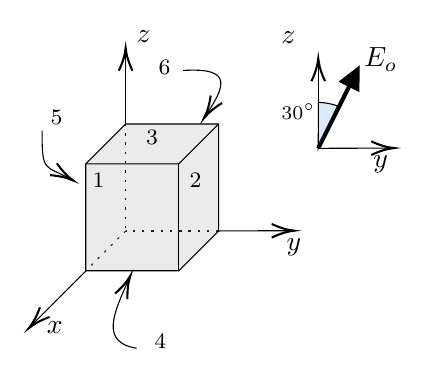
\begin{tikzpicture}[x=0.75pt,y=0.75pt,yscale=-1,xscale=1]
%uncomment if require: \path (0,182); %set diagram left start at 0, and has height of 182

%Straight Lines [id:da9444440815278121] 
\draw  [dash pattern={on 0.84pt off 2.51pt}]  (67.2,109.8) -- (48,129) ;
%Straight Lines [id:da08991584597208946] 
\draw  [dash pattern={on 0.84pt off 2.51pt}]  (112,109.8) -- (67.2,109.8) ;
%Shape: Cube [id:dp7165941380397529] 
\draw  [fill={rgb, 255:red, 155; green, 155; blue, 155 }  ,fill opacity=0.2 ] (48,77.45) -- (67.2,58.25) -- (112,58.25) -- (112,109.8) -- (92.8,129) -- (48,129) -- cycle ; \draw   (112,58.25) -- (92.8,77.45) -- (48,77.45) ; \draw   (92.8,77.45) -- (92.8,129) ;
%Straight Lines [id:da8844067166176446] 
\draw  [dash pattern={on 0.84pt off 2.51pt}]  (67.2,58.25) -- (67.2,109.8) ;
%Straight Lines [id:da20318238488315155] 
\draw    (48.17,129) -- (21.91,155.25) ;
\draw [shift={(20.5,156.67)}, rotate = 315] [color={rgb, 255:red, 0; green, 0; blue, 0 }  ][line width=0.75]    (10.93,-3.29) .. controls (6.95,-1.4) and (3.31,-0.3) .. (0,0) .. controls (3.31,0.3) and (6.95,1.4) .. (10.93,3.29)   ;
%Straight Lines [id:da381549205527151] 
\draw    (112,109.8) -- (146.5,109.67) ;
\draw [shift={(148.5,109.67)}, rotate = 179.79] [color={rgb, 255:red, 0; green, 0; blue, 0 }  ][line width=0.75]    (10.93,-3.29) .. controls (6.95,-1.4) and (3.31,-0.3) .. (0,0) .. controls (3.31,0.3) and (6.95,1.4) .. (10.93,3.29)   ;
%Straight Lines [id:da7722721770942105] 
\draw    (67.2,58.25) -- (67.2,23.67) ;
\draw [shift={(67.2,21.67)}, rotate = 90] [color={rgb, 255:red, 0; green, 0; blue, 0 }  ][line width=0.75]    (10.93,-3.29) .. controls (6.95,-1.4) and (3.31,-0.3) .. (0,0) .. controls (3.31,0.3) and (6.95,1.4) .. (10.93,3.29)   ;
%Straight Lines [id:da5631211047119826] 
\draw [line width=1.5]    (160,70) -- (178.21,33.58) ;
\draw [shift={(180,30)}, rotate = 116.57] [fill={rgb, 255:red, 0; green, 0; blue, 0 }  ][line width=0.08]  [draw opacity=0] (11.61,-5.58) -- (0,0) -- (11.61,5.58) -- cycle    ;
%Straight Lines [id:da8365830796273075] 
\draw    (160,70) -- (194.5,69.87) ;
\draw [shift={(196.5,69.87)}, rotate = 179.79] [color={rgb, 255:red, 0; green, 0; blue, 0 }  ][line width=0.75]    (10.93,-3.29) .. controls (6.95,-1.4) and (3.31,-0.3) .. (0,0) .. controls (3.31,0.3) and (6.95,1.4) .. (10.93,3.29)   ;
%Straight Lines [id:da723347067453898] 
\draw    (160,70) -- (160,28.71) ;
\draw [shift={(160,26.71)}, rotate = 90] [color={rgb, 255:red, 0; green, 0; blue, 0 }  ][line width=0.75]    (10.93,-3.29) .. controls (6.95,-1.4) and (3.31,-0.3) .. (0,0) .. controls (3.31,0.3) and (6.95,1.4) .. (10.93,3.29)   ;
%Curve Lines [id:da5238293302801402] 
\draw    (72.5,166.32) .. controls (55.04,163.41) and (61.1,150.15) .. (68.78,132.93) ;
\draw [shift={(69.5,131.32)}, rotate = 113.96] [color={rgb, 255:red, 0; green, 0; blue, 0 }  ][line width=0.75]    (10.93,-3.29) .. controls (6.95,-1.4) and (3.31,-0.3) .. (0,0) .. controls (3.31,0.3) and (6.95,1.4) .. (10.93,3.29)   ;
%Curve Lines [id:da09178764187978072] 
\draw    (26.93,61.49) .. controls (26.93,81.65) and (27.85,77.85) .. (40.31,84.59) ;
\draw [shift={(41.93,85.49)}, rotate = 209.74] [color={rgb, 255:red, 0; green, 0; blue, 0 }  ][line width=0.75]    (10.93,-3.29) .. controls (6.95,-1.4) and (3.31,-0.3) .. (0,0) .. controls (3.31,0.3) and (6.95,1.4) .. (10.93,3.29)   ;
%Curve Lines [id:da7842102460481515] 
\draw    (94.93,32.49) .. controls (119.89,30.85) and (114.44,40.92) .. (106,53.86) ;
\draw [shift={(104.93,55.49)}, rotate = 303.27] [color={rgb, 255:red, 0; green, 0; blue, 0 }  ][line width=0.75]    (10.93,-3.29) .. controls (6.95,-1.4) and (3.31,-0.3) .. (0,0) .. controls (3.31,0.3) and (6.95,1.4) .. (10.93,3.29)   ;
%Shape: Pie [id:dp592809949302014] 
\draw  [fill={rgb, 255:red, 74; green, 144; blue, 226 }  ,fill opacity=0.2 ] (160.07,47.86) .. controls (160.42,47.87) and (160.78,47.88) .. (161.14,47.9) .. controls (164.05,48.05) and (166.82,48.65) .. (169.36,49.62) -- (160,70) -- cycle ;

% Text Node
\draw (50,80.85) node [anchor=north west][inner sep=0.75pt]  [font=\footnotesize]  {$1$};
% Text Node
\draw (96.8,80.85) node [anchor=north west][inner sep=0.75pt]  [font=\footnotesize]  {$2$};
% Text Node
\draw (75.87,59.77) node [anchor=north west][inner sep=0.75pt]  [font=\footnotesize,rotate=-0.7]  {$3$};
% Text Node
\draw (28,152.4) node [anchor=north west][inner sep=0.75pt]    {$x$};
% Text Node
\draw (143.5,112.07) node [anchor=north west][inner sep=0.75pt]    {$y$};
% Text Node
\draw (71.25,12.13) node [anchor=north west][inner sep=0.75pt]    {$z$};
% Text Node
\draw (141,47.4) node [anchor=north west][inner sep=0.75pt]  [font=\scriptsize]  {$30^{\circ }$};
% Text Node
\draw (185.25,72.4) node [anchor=north west][inner sep=0.75pt]    {$y$};
% Text Node
\draw (141,12.47) node [anchor=north west][inner sep=0.75pt]    {$z$};
% Text Node
\draw (181,20.4) node [anchor=north west][inner sep=0.75pt]    {$E_{o}$};
% Text Node
\draw (79.87,158.42) node [anchor=north west][inner sep=0.75pt]  [font=\footnotesize,rotate=-0.7]  {$4$};
% Text Node
\draw (29.87,50.42) node [anchor=north west][inner sep=0.75pt]  [font=\footnotesize,rotate=-0.7]  {$5$};
% Text Node
\draw (81.87,26.42) node [anchor=north west][inner sep=0.75pt]  [font=\footnotesize,rotate=-0.7]  {$6$};


\end{tikzpicture}


Find the flux through the six labeled faces of the cube with side length $a$ when the electric field is as shown in the diagram.

\end{document}